\documentclass{article}
\usepackage[utf8]{inputenc}
\usepackage[a4paper, total={8in, 10in}]{geometry}
\usepackage{fontspec}
\setmainfont{TeX Gyre Pagella}
\setsansfont{Montserrat}
\usepackage{xeCJK}
\setCJKmainfont{FandolKai-Regular}
\setCJKsansfont{FandolKai-Regular}
\setCJKmonofont{FandolKai-Regular}
\usepackage{unicode-math}

\usepackage{tikz}

\usepackage{graphicx}
\usepackage{float}

\usepackage{listings}
\usepackage{xcolor}
\lstset{
    numbers=left, 
    numberstyle= \tiny, 
    keywordstyle= \color{ blue!70},
    commentstyle= \color{red!50!green!50!blue!50}, 
    frame=shadowbox, % 阴影效果
    rulesepcolor= \color{ red!20!green!20!blue!20} ,
    % escapeinside=';', % 英文分号中可写入中文
    xleftmargin=2em,xrightmargin=2em, aboveskip=1em,
    framexleftmargin=2em
} 

\title{通用人工智能之梦:从大语言模型开始}
\author{jiafeng5513}
\date{\today}

\begin{document}

\maketitle
\section{序言}
首先得说明,按照笔者个人的观点,以语言模型,尤其是所谓的“大语言模型”作为切入点,尝试理清现代人工智能技术的脉络是一个糟糕的想法。作者本人的求学历程正好伴随着“连接主义AI”的最近一次高潮历程,亲眼见证了以“卷积神经网络”为代表的AI技术从野蛮生长到逐渐具备完善的数学性和可解释性,也经历了神经网络模型的训练从“盲人摸象”到“经验主义”,再到发展出成体系的指导思想。在那个群雄逐鹿的年代,还没有现在这样成熟好用的TensorFlow,PyTorch,我和我的导师一起一行一行的读完了贾扬清的第一版Caffe框架,开启了我自己的Ai之旅。但在今天这样的时候,再去重走当年的老路,未免显得有些傲慢与不合时宜,那我们不妨就从大家最感兴趣也是时下最热门的东西:“大语言模型”入手吧。

要想搞清楚什么是大语言模型,首先要搞清楚什么是语言模型,而面对“语言模型”这四个字,我们应该如何着手去了解它呢?思考过后,我决定先抛出一些问题:
\begin{enumerate}
    \item 我们获取一个语言模型的目的是什么?
    \item 语言模型与其他模型的区别是什么?
    \item 语言模型任务的挑战是什么?
    \item 为什么语言模型都比较大,而且越来越大?
    \item 更基本的,当我们说“模型”这个词的时候,我们想表达的是什么?与之相对的又是什么?
    \item 语言模型需要什么样的计算,这些计算对算力设备提出了哪些要求?
    \item 我们能否回答诸如:“为什么chatgpt看起来那么像我们想像中的人工智能”这样的问题?
    \item 当我们谈论“AI”时,我们是在谈论什么?
\end{enumerate}

这些问题可能并不够专业,或许也没能涵盖你最好奇的一些问题,不过仅仅是作抛砖引玉之用。本文的目标在于尽可能的在不回避任何专业术语和数学的情况下,将以深度学习/人工神经网络为代表的人工智能技术和时下热点:以GPT为代表的大语言模型相关的一些技术介绍给从未接触过此类内容的读者。
本文的余下内容将会如此安排:第2章将会介绍一些基本概念,第3章会以一个小模型为例介绍语言类模型的基础计算和深度学习的基础数学概念,第4章梳理语言模型的发展历程,第5章详细介绍Transformer类模型,未完待续。

\section{重新装备}
对于接触过计算机编程,但没有深度接触过数学和深度学习的朋友来说,他们常常会对深度学习或当下的“AI”产生一些误解:以往我们要编程解决一个问题,大量的代码会直接处理问题本身。我们通常会分析和拆解问题,将其转换为更符合计算机习惯,或者说更容易编程解决的问题,然后通过“自顶向下,逐步求精”的指导思想编写程序。笔者曾经编写过一个五子棋AI,使用的是一种被称为“$\alpha$ - $\beta$ 剪枝”的算法,通过遍历对手的一切可能走法和我们的应手来搜索最优解。这就是一种典型的传统思路,也是作为计算机从业人员最容易想到的方法:将问题转换为暴力搜索问题,然后利用计算机强大的算力和海量的存储能力,并使用一切手段加速暴力过程,例如进行剪枝搜索或者采用分布式并行化算法。五子棋和象棋都可以通过强行堆叠存储器进行完全搜索,有人甚至通过该方法证明了在不使用禁手规则的五子棋游戏中,先行者是必胜的。

但是这种方法是有极限的:有些问题无法抽象为一个暴力搜索问题,或者他的解空间维度过高以至于存储和搜索该空间可能需要无法满足的算力。一个典型的例子就是围棋游戏,极简的规则却拥有巨大的解空间。因此,请朋友们建立一个基础认识:对于大多数深度学习解决的问题,开发他们的工程师并不是在“直接”编程解决问题本身,他们是在描述一种数学系统,并假设这个数学系统能够解答目标问题,然后用某种方法得到或者逼近这个数学系统。因此对于一个识别猫狗的深度学习系统来说,没有人会挖空心思的尝试用代码描述那些区别猫和狗的关键特征。

鉴于深度学习的这种特点,他可能会导致我们大脑原来装备的一些解决问题的方法变得无益,因此,在旅程的开始阶段,需要挑选些特定的武器重新装备我们的大脑。基于各种考虑,我们不妨一同复习一下一些有关与深度学习的知识,以免频繁的遇到需要解释的名词。
\subsection{训练}
深度学习(事实上机器学习类似)可以看作是在“寻找一种函数”,这种函数可能非常复杂,以至于难以通过直接给出表达式的方法获得,也无法通过简单的尝试求解微分方程组的方式得到。但是人们可以相对容易的搜集到大量关于这个目标函数的输入和输出的信息。因此我们并不是没有这个目标函数,而是这个目标函数以一种不太方便使用的形式存在于一个黑盒中(例如这个函数是人类的一种能力,是敌军的通信密码本,或者自然界的一种难以模拟的现象等等)。

出于将一切自动化的这种愿望,我们尝试用某种方法“破解”这个黑盒子,正如在战争时期破解任何密码一样,这项工作需要大量的“密文”和与之对应的“明文”作为研究素材。在我们的场景中,如果破译工作是根据“密文-明文对”来进行,则称为有监督训练,如果我们没有任何一条明文,仅有大量的密文并尝试进行破解,则称为无监督训练(或无监督学习),而更常见的情况下数据通常不是“密文-明文对”形式存在的,而是密文和与明文相关的某种其他东西,例如对敌军的侦察情报。特别的,在我们的场景中,把“密文”称之为语料。

对于“只有密文而没有明文”的这种情况,或许会让一部分不了解密码学和机器学习的朋友感到疑惑:这看起来是完全不可实现的任务。实际上则不然,自然语言中存在着许多人类肉体凡胎难以捕捉到的信息,例如对大量的英文语料进行统计,会发现不同字母出现的频率不同,这种特性不会被简单替换密码所破坏,因此只要收集足够的语料,就能在完全没有明文的情况下破解替换密码。你可能已经发现了,在我们的LLM(Large Language Model,大语言模型)场景下,明文对应着问题,而密文对应着答案,而收集足够多的这种对应关系似乎是一件难以完成的任务,因此我们的任务就很类似于这种“在没有明文对应的情况下尝试破解敌人的密码”。

\subsection{损失函数}
你几乎可以在任何深度学习相关的文章中看到这个词,我们可以简单的把他理解为“训练目标就是要最小化这个函数”。如果你对反向传播之类的概念稍有了解,你应该可以说出这样的话:损失函数的值是训练动力的来源。在我们的例子中,你需要时刻记住一件事:损失函数往往最能说明一个模型到底具有什么能力,或者说他是被训练来干什么的。例如在CV(Computer Vision,计算机视觉)任务中,当你看到一个模型使用了回归性损失函数,你就可以猜测他很可能具有“某个东西在某个位置”这样的能力。

具体来说,训练数据从模型的“入口”进入,经历各种运算,从“出口”返回一些数值,我们需要一个方法代替人来评判这些返回的数值是否正确,这便是损失函数。一般地,损失函数值越大,意味着模型返回的数值距离我们想要的样子越远,那就需要根据这个损失值对模型进行调整,这种调整是通过一种被称为“反向传播”的方法进行的。当损失函数值总是很小的时候,训练就会变慢甚至停止,这个时候我们就说这个模型可以收敛。

\subsection{涌现性}
这个词被应用来形容LLM的某种能力。让我先尝试解释他原本的含义:简单的来说就是“量变引发质变”,但请大家注意的,通常量变引发质变会被用在这样的一个场景下:父母教导孩子,刷一万遍做错的题就再也不会做错了,就像你几乎不可能算错1+1那样。请注意这个不是“涌现”,涌现指的是大量被简单规则支配的客体的集合能够表现出超越支配个体的简单规则的性质的一种现象。

比如蚂蚁和蜜蜂的个体行为模式极其简单,但是蚁群和蜂群能够表现出“真社会性”。组成板凳和计算机甚至太阳的质子和中子没有不同,但是他们所构成的物体却有截然不同的理化性质。游戏《我的世界》中仅仅规定了一些基本的物理规则,但是玩家能利用这些符合真实物理法则的小方块在游戏里造出芯片和计算机。在我们的例子中,涌现性指的是:我们用极其简单的约束进行模型的训练,但是模型表现出了一些复杂特性,这些特性并不包含在我们明确提供的约束中。例如我们仅仅要求一个模型尽可能的对于一句上文给出一个通顺的下文,却发现这个模型似乎具备了“回答问题”的能力。

\subsection{Embedding}
这是一个稍微有点复杂的概念,但却是几乎一切现代语言模型的基石。尝试思考这样的一个问题:我们现在有一个英文语料库,英文是由单词组成句子的,英文单词的总量可能是很大的(我估计远大于一百万,因为在我上初中的时候看过一条新闻,第一百万个单词:web2.0诞生了),我们的模型应当有能力认识并输出语料库中的任何一个单词,那么可以想象把每个单词按照字典序列编一个从1到一百万的唯一数字,再把原来的句子替换成这个数字,这样看起来更像是一个能被数学系统处理的东西了。

但是且慢,这里存在一个显而易见的问题:你不能让这个编号直接参与计算,因为这意味着字典序靠后的单词带有一个超级大的数字,这可能会带来两个棘手的问题:
\begin{enumerate}
    \item 我们的模型可能非常复杂,输入数据要经过很多次运算,那么对于一百万这样的数字,就要考虑溢出的风险;
    \item 数值的大小很可能会导致模型更青睐于输出那些字典序靠后/靠前(这却决于损失函数的构造)的单词,我们把这种现象一般称为“退化”,也就是模型在损失函数的约束下找到了一种能最小化损失值的捷径,导致损失函数没能像我们想像的那样引导模型走向正确的方向。
\end{enumerate}

对于问题1,CV任务中常用的诸如归一化之类的方式是有害的,因为这可能会快速的破坏掉语料原本的结构信息(例如“我想出苹果”和“我想吃香蕉”这两句话本来是很类似的,但是苹果这个词的编码是18,香蕉这个词的编码是114514,归一化之后,这两句话看起来可能就不那么相似了)。而对于问题2,看似能够通过设计更好的损失函数来实现,实则不然,过于复杂的损失函数往往并不是一个好的主意,况且这也更难设计。

出于“平等的表示字典中的每一个单词”和“避免出现大小悬殊的数值”这两个目的,我们可能会想到使用“onehot”编码。想象一个语料库中含有$K$个单词,其中第$k$个单词就用一个只有第$k$位为1,其他$K-1$位都为0的向量表示。这个方法就能完美的解决上述两个问题,只不过他会浪费大量的存储空间,尤其是K通常都特别大,随着语料库的扩展,单单是这种向量构成的句子,就会很快超过任何一种已知的GPU的显存的大小,并以不那么令人愉快的方式继续充满主存和外存,直到给想处理它们的程序带来灾难。

因此,我们希望能够找到一种方法,把超级长的这种onehot编码组成的矩阵压缩成一个固定大小的向量,并且不损失其中携带的信息。我并不想在这里展开embedding的具体计算方法,读者在这里只需要知道,我们成功的找到了这么一种方法,能够把那个很夸张的K列的矩阵压缩到很小,这个操作就叫embedding,有的时候这种操作的结果被叫做embedding,有的时候这种操作所需的那个“查找表”被称为embedding,希望读者在看其他论文的时候不会因此而困惑。

\subsection{没有免费的午餐}
这其实是一个看起来很吓人的数学“定理”,但是他的内涵很简单:如果把所有的模型的性能在所有的数据集上做统计,那么他们将会表现出相似的性能。但是如果知道数据集的先验知识,就可以显著提升某些模型在其上的性能。换句话说,不存在一个什么都能干且什么都干的很好的模型。对于这个说法,目前已经有了一种不同的声音,认为该理论已经“过时”了。此处并不像过多的讨论该话题,作为早期的一种说法,我认为并不能给深度学习带来什么新的东西,但鉴于部分“chatgpt将会终结一切深度学习,杀死比赛,降维打击”的说法,我认为有必要保持某种冷静。

\subsection{数据的分布}
在机器学习中,你永远会面对一个问题:无论你的数据集有多大多全面,它永远是真实世界的过去时,永远会有你的模型从来没见过的东西出现。对于这个问题,你可以期待模型拥有“随机应变”的能力,我们称之为泛化能力,泛化能力越好的模型在测试集上的性能越接近训练和验证集。

顺便解释一下这里提到的几个词。训练集(training set)一般比较大,顾名思义就是参与反向传播的那些数据,每次会有一些数据同时进入模型,这些数据被称为一个Batch,所有的训练数据都经过一次模型叫一个Epoch,一般每隔一些Batch,会用一个验证集(validation set)进行推理,并且记录推理时的各种参数,这些被记录的参数一般是用来调整模型的超参(hyper Parameters),超参指的是不被反向传播所修正的那些参数,与之对应的会被反向传播修正的参数就称为可学习/可训练参数。测试集指的是当模型训练结束了,用来测试模型的性能的数据。测试集不能参与过训练,因为这样能够更真实的反应模型的使用状态。而一般来讲提到模型的性能,特指模型的准确率,或者说精度,因为在学术论文里模型的“精度”一般会用若干种指标来衡量,这些指标都是衡量这个模型的输出结果是否能令人满意的,这些统称为性能。在涉及到运行速度的场合会直接说速度或者效率。

回到数据分布的问题上。为了提高泛化性能,可以不停的补充数据进行微调训练(fine turning),几乎所有的商用模型都在不停的干这件事,但更重要的是理解“同分布”的概念。我们提出两个基本假设:1.对于任何有意义的任务,他可能出现的输入数据是符合某种分布的;2.我们能够收集一个有限数据集,使得该数据集与真实数据同分布。在这样的假设下我们可以相信:我们的模型一旦在此数据集上成功训练,能够在真实数据上获得接近训练效果的使用效果。那么什么是“同分布”呢?一个简单替换密码和他的明文是同分布的,同一个城市采集的交通实况录像是同分布的,而在非洲草原拍摄的野生动物照片和在热带雨林拍摄的野生动物照片可能就不是同分布的。实际上学界已经有很多颇具数学性的方法可以进行判定,如果你熟悉机器学习,应该会感觉这种判定类似于一种叫“聚类”的任务。数据集的分布状态对模型性能的影响是非常大的,如果你尝试训练自己的模型,一定要注意这个问题,如果遇到了不明原因的模型性能下降,或许也和这个问题有关。

\subsection{一切都是信息,一切关于信息}
了解相对论和近现代物理学的读者应该对光速是本宇宙的速度上限这件事有所印象。但如果你了解的更多一点,就会知道事实上存在很多“超光速”现象,但这些现象有一个共同点:无法传递任何信息。进入现代,越来越多的现象和研究暗示着一个令人深思的可能性:相比于物质和能量,信息才是第一位的。

对于深度学习系统来说,我们需要时刻把握住一件非常重要的事:

\textbf{信息不能凭空产生,他只能从一种形式转换为另一种形式,信息需要载体才能存在,信息一旦灭失和耗散就无法还原}。

比如对一张图片做pooling,每个四像素邻域取一个最大值保留,这张图片就会缩小,其中max这个操作就会导致信息灭失,即使我们在pooling时保存那个最大值的原始位置,也不可能再还原灭失掉的信息,此时复原原图是不可能的。但请注意,信息灭失不一定是坏事,深度学习系统总归是要为人类服务的,例如一个分类模型可以识别一张照片里的小动物是猫还是狗,输入了一张图片,但是只输出了1bit的信息,有大量的信息灭失掉了,但是却达到了使用者的目的。控制信息的转换和压缩是设计一个深度学习系统的要点:在适当的时候迫使信息进入你想要的维度,在适当的时候通过灭失信息迫使模型舍弃你不需要的东西。

这些话看起来非常抽象,似乎也没什么具体的指导价值,但请相信我,事实并非如此。

\section{数学很重要}
本文致力于给从未涉足过深度学习和机器学习的朋友一个入门级的科普。虽然数学公式的数量和读者的兴趣成负相关,但是AI是一件复杂的事情,我们应该要尽可能的理解“如果一个人说他在做深度学习,那么他每天都在想什么”这样的一个问题。这里的症结在于,对于更多喜欢谈论“AI会如何取代原画设计师,AI会如何让某些职业消失”的人来说,他们谈论的AI更多的是一种抽象的概念,是一个“无所不知的愚蠢的机器人”或者是一个“包含了巨大数据库的含有很多if-else的程序”,我相信其中相当数量的人甚至对于了解其中的具体细节有抵触心理。

但我们不能这样流于表面,如果不了解细节,那些纷繁复杂的关于AI的吹捧可能会让你做出错误的判断。如果清楚了其中的数学把戏,你将会更加容易理解那些自称为“数据科学家”和“高性能计算工程师”的人是如何判断一个模型的性能瓶颈和它将会面临哪些挑战的,也会对那些涉及到AI的未来发展,甚至我们距离通用人工智能还有多远之类的问题有更多自己的见解。

我决定使用一个叫做“DLRM”的模型来做为例子。这个模型是一个推荐系统模型,他缺少语言模型常用的transformer和循环结构,但它具有embedding和interaction等结构,足够简单也足够用于展示相关的数学计算。请大家注意,虽然这个模型是一个看起来非常简单的模型,但是他依然会面临很多可怕的挑战,在这一点上,LLM也是类似的。你可能会看过一些神经网络的图示,有一些模型看起来非常复杂和巨大,但是他其中含有的计算却并不那么困难,而另一些模型的结构看起来紧凑,但却具有令人无法相信的巧思和困难:不要以貌取人。

\subsection{DLRM简介}
DLRM是facebook推出的基于深度学习的推荐系统模型(Deep Learning Recommendation Model)。该模型的任务是,给定一个人的浏览记录,和一个新的网页,判断这个人会不会对这个新的网页感兴趣。为此我们搜集了某人连续24天的数据,每行为一条数据,label、dense、sparse依次排列。label是一个int,dense是最多13个int,其中可能有空值,sparse是最多26个int,其中可能有空值。dense数据的取值范围有限,sparse的取值范围非常大。dense和sparse描述一个网页或者一个视频音乐等等互联网服务,label表示这个人的感兴趣与否。

\subsection{arch}
\begin{figure}[H]
    \centering
    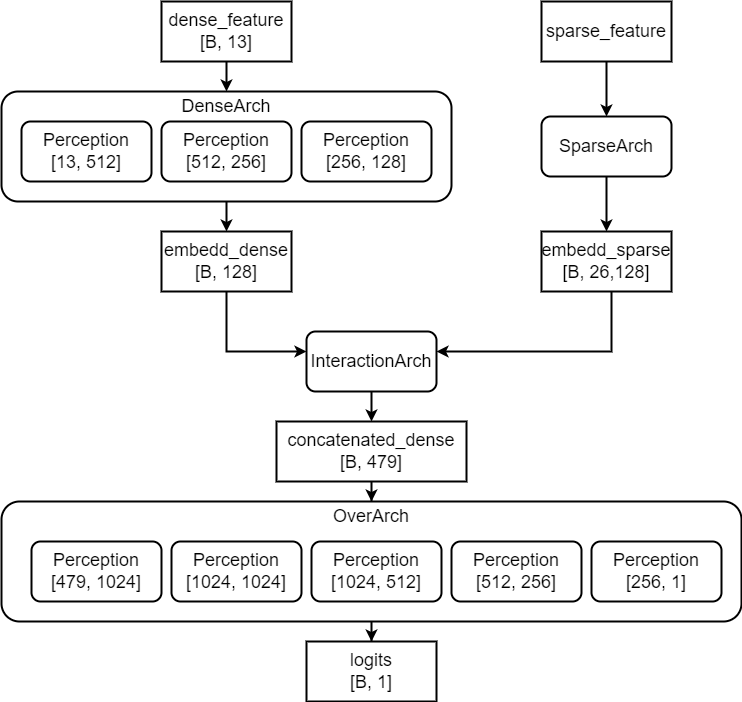
\includegraphics[scale=0.4]{dlrm2_arch.png}
    \caption{dlrm arch}
\end{figure}

\subsection{数据处理}
\begin{enumerate}
    \item 把label,dense,sparse分开,空值用0填充。
    \item $dense = ln(dense+3)$,转为float32存储。
    \item sparse每一列单独处理,转换为连续数字,即每出现一个不同的数字,就替换为id,同时id+1,每遇到一个已经出现过的数字,就换成它第一次出现时使用的id。id从2开始。
    \item 打乱day\_0到day\_22,作为训练集,保留day\_23作为测试集。
    \item 向模型供给数据时,dense和label直接供给,sparse转换为KeyedJaggedTensor。
\end{enumerate}
KeyedJaggedTensor:
\begin{enumerate}
    \item value:sparse$[B, 26]$ 列优先存储成一维。
    \item offset:list, $form\ 0\ to batch\_size*26+1$。
    \item stride: $batch\_size$。
    \item length: list, $batch\_size*26$个1。
    \item key:list of string,from cat\_0 to cat\_25。
    \item length\_per\_key: list,26个$batch\_size$。
    \item offset\_per\_key: list,list $[from\ 0\ to\ 26] * batch\_size$。
    \item 方法to\_dict():返回要给dict,keys from cat\_0 to cat\_25,value有三个字段:
    \begin{itemize}
        \item \_values是一个一维tensor,就是原始的sparse对应cat\_x的那一列值
        \item \_length是一个长度为batch\_size的一维tensor,都是1,
        \item \_offset是一个长度为batch\_size+1的一维tensor,从0到batch\_size
    \end{itemize}
\end{enumerate}
如果使用mulit\_hot\_embedding,供给给后端的sparse数据会经过二次处理,该处理的具体过程如下:
\begin{enumerate}
    \item 初始化需要额外的超参数:
    \begin{itemize}
        \item $multi\_hot\_min\_table\_size$:只有那些$num\_embedding>=multi\_hot\_min\_table\_size$的$sparse\_feature$会经历额外处理。
        \item $multi\_hot\_size$:被额外处理的那些sparse\_feature,被处理之前是$[batch\_size,]$,处理完了是$[batch\_size*multi\_hot\_size,]$。
        \item $collect\_multi\_hot\_freqs\_stats$:是否统计频率。
        \item $multi\_hot\_distribution\_type$:初始化$weight$用的分布模式。
    \end{itemize}
    \item 初始化$weight$:$weight[i]$是一个$shape=[num\_embeddings[i], multi\_hot\_size]$的矩阵,使用$i$作为随机数种子,使用超参指定的分布进行初始化。
    \item 初始化$offset\_n$:
    \begin{enumerate}
        \item 总长度是$num\_sparse\_features*batch\_size+1$。
        \item 初始化一个$lso = ones(sparse\_features\_num * batch\_size)$。
        \item $if\ feature[i]\ has\ num\_embedding >= multi\_hot\_min\_table\_size, lso[i*B : (i+1)*B] = multi\_hot\_size$。
        \item 在$lso$的最前面加一个0。
        \item $offset\_n[0] = lso[0], offset\_n[i] = lso[i] + offset\_n[i-1]$。
    \end{enumerate} 
    \item 处理数据
    \begin{enumerate}
        \item 设转换完的数据为$ls\_n$,转换前的数据为$ls\_i$,注意$ls\_i.shape=[num\_sparse\_features, batch\_size]$。
        \item 如果$num\_embeddings[i]<multi\_hot\_min\_table\_size$,则$ls\_n[i] = ls\_i[i]$,注意$shape=[batch\_size,]$。
        \item 如果$num\_embeddings[i]>=multi\_hot\_min\_table\_size$,则$ls\_n[i] = mulit\_hot\_i$,注意$shape=[batch\_size*multi\_hot\_size,]$。
        \item $mulit\_hot = torch.nn.functional.embedding(ls\_i[i], weight[i])$,$shape=[batch\_size, multi\_hot\_size]$。
        \item 把第一列替换为原始的sparse:$mulit\_hot[,0] = ls\_i[i]$。
        \item $mulit\_hot\_i = mulit\_hot.rehsape(-1)$,更新$ls\_n[i]$。
        \item 此时如果需要统计频率,则分别计数$ls\_n[i]$和$ls\_i[i]$中unique的元素的数量,设频率计数数组为freq,则freq有$num\_sparse\_features$行,每行中存储一个数组,记录$feature[i]$中unique元素出现的数量,处理前后分别统计。
        \item 把$ls\_n$转换成一维的。
    \end{enumerate}
    \item 用$ls\_n$替换dataloader的sparse.values,用$offset\_n$替换dataloader的sparse.offset。
    \item mulit\_hot处理有什么效果:
    \begin{enumerate}
        \item 一个batch里面仍然含有$num\_sparse\_features*batch\_size$个sparse feature。
        \item 对于某些feature,它可能有巨大的取值范围,我们给取值范围设置了一个阈值。
        \item 对于那些取值范围在阈值之下的feature,它传给后端的每一个单独的sparse feature就是一个数,和以前一样。
        \item 对于那些取值范围在阈值之上的feature,我们预先对他进行了一步embedding,转成了我们设置好的一个的长度。
        \item 对于那些经历过额外的embedding的feature,它传给后端的每一个单独的sparse feature是多个数。
        \item 因为有些sparse feature是多个数,因此offset是不均匀的,在没经历过变换的区段,相邻的offset差值为1,而在经历过变换的区段,相邻的offset之间差$multi\_hot\_size$。
        \item 虽然统计了频率,不过除了把频率保存成文件之外,并没有任何其他的用途。
        \item 此处的embedding的weight是无法更新的。
    \end{enumerate}
\end{enumerate}
举个例子:\newline
设$B=2$,$sparse\_features\_num = 4$, 这四个feature的$num\_embeddings=[6,7,5,9]$,\newline$multi\_hot\_min\_table\_size = 8$。
$multi\_hot\_size=3$.我们取一个batch的数据:
$$
\begin{bmatrix}
    I_{0,0} & I_{0,1} & I_{0,2} & I_{0,3} \\\\
    I_{1,0} & I_{1,1} & I_{1,2} & I_{1,3}
\end{bmatrix}
$$
在KeyedJaggedTensor中,value字段是列优先存储的:
$$
[I_{0,0}, I_{1,0}, I_{0,1}, I_{1,1}, I_{0,2}, I_{1,2}, I_{0,3}, I_{1,3}]
$$
对应的offset是:
$$
[0, 1, 2, 3, 4, 5 ,6, 7, 8]
$$
根据规则,第4列会被额外处理,因为第4列的$num\_embeddings=9>multi\_hot\_min\_table\_size=8$,前3列会保持不变。\newline
现在来看怎么处理这个第四列。为了做这个处理,需要先初始化weight[9, 3],9是因为这一列feature的$num\_embeddings=9$,3是因为$multi\_hot\_size=3$,初始化使用的随机数种子是3,因为这个feature在4个sparse feature中的下标是3。$w_{i,j}\in [0,9)$:\newline
$$
weight = 
\begin{bmatrix}
    w_{0,0} & w_{0,1} & w_{0,2} \\\\
    w_{1,0} & w_{1,1} & w_{1,2} \\\\
    w_{2,0} & w_{2,1} & w_{2,2} \\\\
    w_{3,0} & w_{3,1} & w_{3,2} \\\\
    w_{4,0} & w_{4,1} & w_{4,2} \\\\
    w_{5,0} & w_{5,1} & w_{5,2} \\\\
    w_{6,0} & w_{6,1} & w_{6,2} \\\\
    w_{7,0} & w_{7,1} & w_{7,2} \\\\
    w_{8,0} & w_{8,1} & w_{8,2} 
\end{bmatrix}
$$
计算$torch.nn.functional.embedding([I_{0,3}, I_{1,3}], weight)$,因为输入两个元素,$weight.shape=[9,3]$,所以输出是一个$shape=[2,3]$的矩阵:(第4列有$batch\_size$个元素,处理完了会有$batch\_size*multi\_hot\_size$个元素)。然后把这个输出的矩阵的第一列,再替换成输入的值:
$$
\begin{bmatrix}
    I_{0,3} \\\\
    I_{1,3}
\end{bmatrix}
\stackrel{torch.nn.functional.embedding}{\longrightarrow}
\begin{bmatrix}
    I_{0,3}^0 & I_{0,3}^1 & I_{0,3}^2 \\\\
    I_{1,3}^0 & I_{1,3}^1 & I_{1,3}^2 
\end{bmatrix}
\stackrel{replace\ first\ col\ with\ input}{\longrightarrow}
\begin{bmatrix}
    I_{0,3} & I_{0,3}^1 & I_{0,3}^2 \\\\
    I_{1,3} & I_{1,3}^1 & I_{1,3}^2 
\end{bmatrix}
$$
此时这个batch的数据就变成了这样,注意,这仍然是一个2\times4的矩阵,只不过其中两个元素从1个数字变成了3个数字:
$$
\begin{bmatrix}
    I_{0,0} & I_{0,1} & I_{0,2} & I_{0,3} \\\\
    \       & \       & \       & I_{0,3}^1 \\\\
    \       & \       & \       & I_{0,3}^2 \\\\
    I_{1,0} & I_{1,1} & I_{1,2} & I_{1,3} \\\\
    \       & \       & \       & I_{1,3}^1 \\\\
    \       & \       & \       & I_{1,3}^2
\end{bmatrix}
$$
在KeyedJaggedTensor中,value字段是列优先存储的:
$$
[I_{0,0}, I_{1,0}, I_{0,1}, I_{1,1}, I_{0,2}, I_{1,2}, I_{0,3}, I_{0,3}^1, I_{0,3}^2, I_{1,3}, I_{1,3}^1, I_{1,3}^2]
$$
对应的offset是:
$$
[0, 1, 2, 3, 4, 5 ,6, 9, 12]
$$

并且值得注意的是,$[I_{0,3}, I_{1,3}]$的取值范围和$[I_{0,3}^0, I_{0,3}^1, I_{0,3}^2, I_{1,3}^0, I_{1,3}^1, I_{1,3}^2]$的取值范围完全一样,都是$[0, 9)$。那么经历了这个处理之后,这一个batch中含有的sparse\ feature是不是变多了呢?答案是没变,但是有些feature从"single hot"变成了"multi hot"。
\paragraph*{}全局来看,multi hot处理能起到什么作用呢?可以肯定的是,这种处理并不能在任何地方减少计算量或者存储量。因为将"single hot"变成"multi hot"的那一步embedding所用的查找表的仍然是按照该feature原来的取值范围取值的,没有起到压缩index范围的效果,并且在这一步之后还直接拼接了原始的feature,那么这样的结果,就会造成后端的embedding产生额外的查找和计算,而且由于取值范围没有压缩,后端的embedding使用的查找表体积也不能减小。

\subsection{DenseArch and OverArch}
实际上就是nn.Linear和torch.relu堆叠而成的全连接层。

\section{SparseArch}
SparseArch forward: (see def of class SparseArch in dlrm.py line 35)
\begin{enumerate}
    \item KeyedJaggedTensor格式的sparse作为输入,注意features在values字段中,长度是$batch\_size * 26$.
    \item SparseArch初始化需要一个$embedding\_bag\_collection$,这是一个算子,要先初始化它,它的初始化需要"list of EmbeddingBagConfig",长度是26。
    \item EmbeddingBagConfig包含sparse feature对应那一列的$num\_embeddings$(就是超参里那个),$embedding\_dim$(就是那个128),$name(t\_cat\_{from\ 0\ to\ 26-1})$, $feature\_names(cat\_{form\ 0\ to 26-1})$, $pooling\ type(sum)$。
    \item 计算的第一步就是把输入的KeyedJaggedTensor格式的sparse传给$embedding\_bag\_collection$算子处理(see embedding\_modules.py line 67)。
    \begin{itemize}
        \item $embedding\_bag\_collection$算子首先遍历"list of EmbeddingBagConfig",然后创建$module\_dict$, key是EmbeddingBagConfig的name,value是一个torch.nn.EmbeddingBag。
        \item 对于每一个torch.nn.EmbeddingBag,他需要$num\_embeddings$,$embedding\_dim$,$mode$等参数进行初始化,其中$mode$就是EmbeddingBagConfig中的pooling type(也就是sum),其他值你会发现EmbeddingBagConfig中也都有。
        \item 调用输入sparse的$to\_dict$方法,返回值为$feature\_dict$。
        \item 然后再遍历$feature\_dict$,用$key$查询$module\_dict$,获得初始化好的对应的torch.nn.EmbeddingBag算子,然后调用他的即forward,所需的参数为$input$即$\_values$, $offsets$即$\_offset$(注意长度为$batch\_size+1$)。
        \item 到这里其实就是对于$sparse$的每一列使用了torch.nn.EmbeddingBag,每一列返回一个$[batch\_size, 128]$, 一共26列,concat到一起就是$[batch\_size, 3328=26*128]$。
        \item 然后构造一个KeyedTensor对象,其中key字段是$cat\_{form 0 to 26-1}$, values字段就是$[batch\_size, 3328=26*128]$, $length\_per\_key$字段是长度为26的list,值都是128,就是每一个embeddingBag的embedding dim。
        \item 返回KeyedTensor对象。
    \end{itemize}
    \item 第二步
    \begin{itemize}
        \item 调用KeyedTensor对象的$to_dict()$,把$value$从$dim=1$上切成26个$[batch\_size, 128]$,
        \item 把26个$[batch\_size, 128]$在$dim=1$上concat
        \item $reshape$成$[batch, 26, 128]$
    \end{itemize}
\end{enumerate}

\section{EmbeddingBag inside}
在这个例子中我们有:
$$X=
\left[
    \begin{array}{ccc}
        x_{0,0} & x_{0,1} &x_{0,2}\\\\
        x_{1,0} & x_{1,1} &x_{1,2}\\\\
    \end{array}
\right],W=
\left[
    \begin{array}{ccc}
        w_{0,0} & w_{0,1} & w_{0,2}\\\\
        w_{1,0} & w_{1,1} & w_{1,2}\\\\
        w_{2,0} & w_{2,1} & w_{2,2}\\\\
        w_{3,0} & w_{3,1} & w_{3,2}\\\\
    \end{array}
\right]$$
$$batch\_size=2, num\_embedding=4, embedding\_dim=3, K=3$$
$$W.shape=\left[num\_embedding, embedding\_dim\right]$$
$$X.shape=\left[batch\_size, K\right]$$
$$for\ each\ x_{i,j}\ in\ X, x_{i,j} \in [0, num\_embedding-1]$$
需要指出,对于如果采用了multi\_hot处理,$X$的某些值可能是由多个值组成的,但为了推导方便我们不妨假设每一个$x$都恰好只含有一个值,实际上由于EmbeddingBag包含一个求和操作,这个假设并不会造成推导结果与实际情况区别过大。

则EmbeddingBag forward:
$$Y_{i,j}=\sum_{k=0}^K{w_{x_i,k},j}$$

对于EmbeddingBag backward,因为EmbeddingBag是第一层,所以仅需要考虑权重更新。已知:
$$\frac{\partial L}{\partial Y}=
\left[
    \begin{array}{ccc}
        \frac{\partial L}{\partial Y_{0,0}} & \frac{\partial L}{\partial Y_{0,1}} & \frac{\partial L}{\partial Y_{0,2}}\\\\
        \frac{\partial L}{\partial Y_{1,0}} & \frac{\partial L}{\partial Y_{1,1}} & \frac{\partial L}{\partial Y_{1,2}}\\\\
    \end{array}
\right]$$
求:$$\frac{\partial L}{\partial W}$$

从forward中可以看到$Y_{i,j}$是第$j$列某些$W$的和,这些$W$的行数是由第$i$行的$x$的值决定。把Y展开:
$$
Y=
\left[
    \begin{array}{ccc}
        y_{0,0} & y_{0,1} & y_{0,2}\\\\
        y_{1,0} & y_{1,1} & y_{1,2}\\\\
    \end{array}
\right]
=
\left[
    \begin{array}{ccc}
        w_{x_{0,0},0} + w_{x_{0,1},0} + w_{x_{0,2},0} & w_{x_{0,0},1} + w_{x_{0,1},1} + w_{x_{0,2},1} & w_{x_{0,0},2} + w_{x_{0,1},2} + w_{x_{0,2},2}\\\\
        w_{x_{1,0},0} + w_{x_{1,1},0} + w_{x_{1,2},0} & w_{x_{1,0},1} + w_{x_{1,1},1} + w_{x_{1,2},1} & w_{x_{1,0},2} + w_{x_{1,1},2} + w_{x_{1,2},2}\\\\
    \end{array}
\right]
$$
为了更新$W$,我们需要计算:
$$\frac{\partial L}{\partial W}=
\left[
    \begin{array}{ccc}
        \frac{\partial L}{\partial w_{0,0}} & \frac{\partial L}{\partial w_{0,1}} & \frac{\partial L}{\partial w_{0,2}}\\\\
        \frac{\partial L}{\partial w_{1,0}} & \frac{\partial L}{\partial w_{1,1}} & \frac{\partial L}{\partial w_{1,2}}\\\\
        \frac{\partial L}{\partial w_{2,0}} & \frac{\partial L}{\partial w_{2,1}} & \frac{\partial L}{\partial w_{2,2}}\\\\
        \frac{\partial L}{\partial w_{3,0}} & \frac{\partial L}{\partial w_{3,1}} & \frac{\partial L}{\partial w_{3,2}}\\\\
    \end{array}
\right]
$$
以$w_{0,0}$为例,
$$
\frac{\partial L}{\partial w_{0,0}}=\frac{\partial L}{\partial Y} \frac{\partial Y}{\partial w_{0,0}}
$$
其中$\frac{\partial L}{\partial Y}$是已知的,跟据Y的表达式,我们可以计算出$\frac{\partial Y}{\partial w_{0,0}}$:
$$\frac{\partial Y}{\partial w_{0,0}} = 
\left[
    \begin{array}{ccc}
        p_{0,0} & 0 & 0\\\\
        p_{1,0} & 0 & 0\\\\
    \end{array}
\right]
$$
其中$p_{0,0}$是“$x_{0,k}$中x=0的个数”,$p_{1,0}$是“$x_{1,k}$中x=0的个数”。注意在这个案例里$K=3$,在当前的dlrm参考实现中$K$对于每一个feature是一个固定的值,但feature之间具有不同的$K$。$x_{i,k}$代表第$i$行的所有$x$。给$p$一个形式化的定义:
$$p_{n, m}=count_{k}(x_{n,k}=m)$$
然后进一步:
$$
\frac{\partial L}{\partial w_{0,0}}=\frac{\partial L}{\partial Y} \frac{\partial Y}{\partial w_{0,0}}
=
\left[
    \begin{array}{ccc}
        \frac{\partial L}{\partial y_{0,0}} & \frac{\partial L}{\partial y_{0,1}} & \frac{\partial L}{\partial y_{0,2}}\\\\
        \frac{\partial L}{\partial y_{1,0}} & \frac{\partial L}{\partial y_{1,1}} & \frac{\partial L}{\partial y_{1,2}}\\\\
    \end{array}
\right]
\cdot
\left[
    \begin{array}{ccc}
        p_{0,0} & 0 & 0\\\\
        p_{1,0} & 0 & 0\\\\
    \end{array}
\right]
=
\frac{\partial L}{\partial y_{0,0}}p_{0,0} + \frac{\partial L}{\partial y_{1,0}}p_{1,0}
$$
类似的,计算出整个$\frac{\partial L}{\partial W}$:
$$
\frac{\partial L}{\partial W} = 
\left[
    \begin{array}{ccc}
        \frac{\partial L}{\partial y_{0,0}}p_{0,0} + \frac{\partial L}{\partial y_{1,0}}p_{1,0} & \frac{\partial L}{\partial y_{0,1}}p_{0,0} + \frac{\partial L}{\partial y_{1,1}}p_{1,0} & \frac{\partial L}{\partial y_{0,2}}p_{0,0} + \frac{\partial L}{\partial y_{1,2}}p_{1,0}\\\\
        \frac{\partial L}{\partial y_{0,0}}p_{0,1} + \frac{\partial L}{\partial y_{1,0}}p_{1,1} & \frac{\partial L}{\partial y_{0,1}}p_{0,1} + \frac{\partial L}{\partial y_{1,1}}p_{1,1} & \frac{\partial L}{\partial y_{0,2}}p_{0,1} + \frac{\partial L}{\partial y_{1,2}}p_{1,1}\\\\
        \frac{\partial L}{\partial y_{0,0}}p_{0,2} + \frac{\partial L}{\partial y_{1,0}}p_{1,2} & \frac{\partial L}{\partial y_{0,1}}p_{0,2} + \frac{\partial L}{\partial y_{1,1}}p_{1,2} & \frac{\partial L}{\partial y_{0,2}}p_{0,2} + \frac{\partial L}{\partial y_{1,2}}p_{1,2}\\\\
        \frac{\partial L}{\partial y_{0,0}}p_{0,3} + \frac{\partial L}{\partial y_{1,0}}p_{1,3} & \frac{\partial L}{\partial y_{0,1}}p_{0,3} + \frac{\partial L}{\partial y_{1,1}}p_{1,3} & \frac{\partial L}{\partial y_{0,2}}p_{0,3} + \frac{\partial L}{\partial y_{1,2}}p_{1,3}\\\\
    \end{array}
\right]
$$
分解:
$$
\frac{\partial L}{\partial W} =
P\frac{\partial L}{\partial Y} = 
\left[
    \begin{array}{ccc}
        p_{0,0} & p_{1,0}  \\\\
        p_{0,1} & p_{1,1}  \\\\
        p_{0,2} & p_{1,2}  \\\\
        p_{0,3} & p_{1,3}  \\\\
    \end{array}
\right]
\left[
    \begin{array}{ccc}
        \frac{\partial L}{\partial Y_{0,0}} & \frac{\partial L}{\partial Y_{0,1}} & \frac{\partial L}{\partial Y_{0,2}}\\\\
        \frac{\partial L}{\partial Y_{1,0}} & \frac{\partial L}{\partial Y_{1,1}} & \frac{\partial L}{\partial Y_{1,2}}\\\\
    \end{array}
\right]
$$
观察$P$,发现$P$的第0列就是$X$的第0行的值中,取得$0,1,2$的元素的数量,因此只需要统计出这个$P$矩阵,就可以更新EmbeddingBag层的weight。

\section{InteractionArch}
一共有三种Interaction备选:
\begin{enumerate}
    \item Default:Returns the pairwise dot product of each sparse feature pair, the dot product of each sparse features with the output of the dense layer, and the dense layer itself (all concatenated).
    \item DCN:Returns the output of a Deep Cross Net v2 https://arxiv.org/pdf/2008.13535.pdf with a low rank approximation for the weight matrix. The input and output sizes are the same for this interaction layer (F*D + D).
    \item Projection: Return Y*Z and the dense layer itself (all concatenated) where Y is the output of interaction branch 1 and Z is the output of interaction branch 2. Y and Z are of size Bx(F1xD) and Bx(DxF2) respectively for some F1 and F2.
\end{enumerate}

\section{Default Interaction}
forward:
\lstset{language=Python}
\begin{lstlisting}
# dense_features.shape = [B, 128]
# sparse_features.shape = [B, 26, 128]
combined_values = 
    torch.cat((dense_features.unsqueeze(1), sparse_features),
              dim=1)
# combined_values.shape = [B, 27, 128]

# [B, 27, 27] = [B, 27, 128] <bmm> [B, 128, 27]
interactions = 
    torch.bmm(combined_values, 
              torch.transpose(combined_values, 1, 2))
# [B, 351]
interactions_flat = 
    interactions[:, self.triu_indices[0], self.triu_indices[1]]

# concatenated_dense.shape = [B, 479]
concatenated_dense = 
    torch.cat((dense_features, interactions_flat), dim=1)
\end{lstlisting}
给forward形式化的表达。为了方便推导,我们假设$B=2$,$embedding\_dim=4$,$sparse\_feature\_size=2$:
$$
D\ for\ dense [2, 4] =
\begin{bmatrix}
    d_{0,0} & d_{0,1} & d_{0,2} & d_{0,3} \\\\
    d_{1,0} & d_{1,1} & d_{1,2} & d_{1,3} \\\\
\end{bmatrix}
$$

$$
S\ for\ sparse [2, 2, 4] =
\begin{bmatrix}
    [s_{0,0,0},s_{0,0,1},s_{0,0,2},s_{0,0,3}] & [s_{0,1,0},s_{0,1,1},s_{0,1,2},s_{0,1,3}] \\\\
    [s_{1,0,0},s_{1,0,1},s_{1,0,2},s_{1,0,3}] & [s_{1,1,0},s_{1,1,1},s_{1,1,2},s_{1,1,3}] \\\\
\end{bmatrix}
$$

$$
C\ for\ Comb [2, 3, 4] =
\begin{bmatrix}
    [d_{0,0},d_{0,1},d_{0,2},d_{0,3}] & [s_{0,0,0},s_{0,0,1},s_{0,0,2},s_{0,0,3}] & [s_{0,1,0},s_{0,1,1},s_{0,1,2},s_{0,1,3}]\\\\
    [d_{1,0},d_{1,1},d_{1,2},d_{1,3}] & [s_{1,0,0},s_{1,0,1},s_{1,0,2},s_{1,0,3}] & [s_{1,1,0},s_{1,1,1},s_{1,1,2},s_{1,1,3}]\\\\
\end{bmatrix}
$$


$$
C^T [2,4,3]=
\begin{bmatrix}
    [d_{0,0},s_{0,0,0},s_{0,1,0}] & [d_{0,1},s_{0,0,1},s_{0,1,1}] & [d_{0,2},s_{0,0,2},s_{0,1,2}] & [d_{0,3},s_{0,0,3},s_{0,1,3}]\\\\
    [d_{1,0},s_{1,0,0},s_{1,1,0}] & [d_{1,1},s_{1,0,1},s_{1,1,1}] & [d_{1,2},s_{1,0,0},s_{1,1,2}] & [d_{1,3},s_{1,0,3},s_{1,1,3}]\\\\
\end{bmatrix}
$$

$$
flat(CC^T)|_{b=\{0,1\}}=
\begin{bmatrix}
      \cdots   &   F_{b,0}     & F_{b,1}  \\\\
      F_{b,0}  &   \cdots      & F_{b,2}  \\\\ 
      F_{b,1}  &   F_{b,2}     & \cdots   \\\\
\end{bmatrix}
$$
其中:
$$
F_{b,0}=d_{b,0}s_{b,0,0}+d_{b,1}s_{b,0,1}+d_{b,2}s_{b,0,2}+d_{b,3}s_{b,0,3}
$$
$$
F_{b,1}=d_{b,0}s_{b,1,0}+d_{b,1}s_{b,1,1}+d_{b,2}s_{b,1,2}+d_{b,3}s_{b,1,3}
$$
$$
F_{b,2}=s_{b,0,0}s_{b,1,0}+s_{b,0,1}s_{b,1,1}+s_{b,0,2}s_{b,1,2}+s_{b,0,3}s_{b,1,3}
$$

$$
Y[2, 7]=
\begin{bmatrix}
    d_{0,0} & d_{0,1} & d_{0,2} & d_{0,3} & F_{0, 0} & F_{0, 1} & F_{0, 2} \\\\
    d_{1,0} & d_{1,1} & d_{1,2} & d_{1,3} & F_{1, 0} & F_{1, 1} & F_{1, 2} \\\\
\end{bmatrix}
$$
backward:
已知$\frac{\partial L}{\partial Y}$,求$\frac{\partial L}{\partial D}$和$\frac{\partial L}{\partial S}$。
$$
\frac{\partial L}{\partial Y} = 
\begin{bmatrix}
    \frac{\partial L}{\partial y_{0,0}} & \frac{\partial L}{\partial y_{0,1}} & \frac{\partial L}{\partial y_{0,2}} & \frac{\partial L}{\partial y_{0,3}} & \frac{\partial L}{\partial y_{0,4}} & \frac{\partial L}{\partial y_{0,5}}& \frac{\partial L}{\partial y_{0,6}} \\\\
    \frac{\partial L}{\partial y_{1,0}} & \frac{\partial L}{\partial y_{1,1}} & \frac{\partial L}{\partial y_{1,2}} & \frac{\partial L}{\partial y_{1,3}} & \frac{\partial L}{\partial y_{1,4}} & \frac{\partial L}{\partial y_{1,5}}& \frac{\partial L}{\partial y_{1,6}} \\\\
\end{bmatrix}
,
\frac{\partial L}{\partial D} = 
\begin{bmatrix}
    \frac{\partial L}{\partial d_{0,0}} & \frac{\partial L}{\partial d_{0,1}} & \frac{\partial L}{\partial d_{0,2}} & \frac{\partial L}{\partial d_{0,3}} \\\\
    \frac{\partial L}{\partial d_{1,0}} & \frac{\partial L}{\partial d_{1,1}} & \frac{\partial L}{\partial d_{1,2}} & \frac{\partial L}{\partial d_{1,3}} \\\\
\end{bmatrix}
$$
以$\frac{\partial L}{\partial d_{0,0}}$为例:
$$
\frac{\partial L}{\partial d_{0,0}} = \frac{\partial L}{\partial Y} \frac{\partial Y}{\partial d_{0,0}} 
=\frac{\partial L}{\partial Y}
\begin{bmatrix}
    1 & 0 & 0 & 0 & s_{0,0,0} & s_{0,1,0} & 0 \\\\
    0 & 0 & 0 & 0 &         0 &         0 & 0 \\\\ 
\end{bmatrix}
=\frac{\partial L}{\partial y_{0,0}}+s_{0,0,0}\frac{\partial L}{\partial y_{0,4}}+s_{0,1,0}\frac{\partial L}{\partial y_{0,5}}
$$
类似的,可以计算出所有的项:
$$
\frac{\partial L}{\partial d_{i,j}}=\frac{\partial L}{\partial y_{i,j}}+s_{i,0,j}\frac{\partial L}{\partial y_{i,4}}+s_{i,1,j}\frac{\partial L}{\partial y_{i,5}}
$$

$$
\frac{\partial L}{\partial D} = \frac{\partial L}{\partial Y}|_{[:,0:4]}+
\begin{bmatrix}
    s_{0,0,0}\frac{\partial L}{\partial y_{0,4}}+s_{0,1,0}\frac{\partial L}{\partial y_{0,5}} & s_{0,0,1}\frac{\partial L}{\partial y_{0,4}}+s_{0,1,1}\frac{\partial L}{\partial y_{0,5}} & s_{0,0,2}\frac{\partial L}{\partial y_{0,4}}+s_{0,1,2}\frac{\partial L}{\partial y_{0,5}} & s_{0,0,3}\frac{\partial L}{\partial y_{0,4}}+s_{0,1,3}\frac{\partial L}{\partial y_{0,5}} \\\\
    s_{1,0,0}\frac{\partial L}{\partial y_{1,4}}+s_{1,1,0}\frac{\partial L}{\partial y_{1,5}} & s_{1,0,1}\frac{\partial L}{\partial y_{1,4}}+s_{1,1,1}\frac{\partial L}{\partial y_{1,5}} & s_{1,0,2}\frac{\partial L}{\partial y_{1,4}}+s_{1,1,2}\frac{\partial L}{\partial y_{1,5}} & s_{1,0,3}\frac{\partial L}{\partial y_{1,4}}+s_{1,1,3}\frac{\partial L}{\partial y_{1,5}} \\\\
\end{bmatrix}
$$

$$
\frac{\partial L}{\partial D} = \frac{\partial L}{\partial Y}|_{[:,0:4]}+
\begin{bmatrix}
    \frac{\partial L}{\partial y_{0,4}} & \frac{\partial L}{\partial y_{0,5}} \\\\
    \frac{\partial L}{\partial y_{1,4}} & \frac{\partial L}{\partial y_{1,5}} \\\\
\end{bmatrix}
S
$$
注意中间这一项的shape是$[2,1,2]$,左乘S之后得到一个$shape=[2,1,4]$,需要把中间的这个维度$squeeze$掉再和第一项相加。
因为Interaction是两个输入,因此还需要计算关于另一个输入的导数:
$$
\frac{\partial L}{\partial S} = 
\begin{bmatrix}
    [\frac{\partial L}{\partial s_{0,0,0}},\frac{\partial L}{\partial s_{0,0,1}},\frac{\partial L}{\partial s_{0,0,2}},\frac{\partial L}{\partial s_{0,0,3}}] & [\frac{\partial L}{\partial s_{0,1,0}},\frac{\partial L}{\partial s_{0,1,1}},\frac{\partial L}{\partial s_{0,1,2}},\frac{\partial L}{\partial s_{0,1,3}}] \\\\
    [\frac{\partial L}{\partial s_{1,0,0}},\frac{\partial L}{\partial s_{1,0,1}},\frac{\partial L}{\partial s_{1,0,2}},\frac{\partial L}{\partial s_{1,0,3}}] & [\frac{\partial L}{\partial s_{1,1,0}},\frac{\partial L}{\partial s_{1,1,1}},\frac{\partial L}{\partial s_{1,1,2}},\frac{\partial L}{\partial s_{1,1,3}}] \\\\
\end{bmatrix}  
$$
以第一项为例:
$$
\frac{\partial L}{\partial s_{0,0,0}} = \frac{\partial L}{\partial Y}\frac{\partial Y}{\partial s_{0,0,0}}
=
\frac{\partial L}{\partial Y}
\begin{bmatrix}
    0 & 0 & 0 & 0 & d_{0,0} & 0 & s_{0,1,0} \\\
    0 & 0 & 0 & 0 &       0 & 0 &         0 
\end{bmatrix}
=d_{0,0} \frac{\partial L}{\partial y_{0,4}} +  s_{0,1,0}\frac{\partial L}{\partial y_{0,6}}
$$
由于S比较长,省略一些中间过程:
$$
\frac{\partial L}{\partial S} = 
\begin{bmatrix}
    A & B \\\\
    C & D 
\end{bmatrix}
$$
其中:
$$
A=
\begin{bmatrix}
    \frac{\partial L}{\partial y_{0,4}} & \frac{\partial L}{\partial y_{0,6}}
\end{bmatrix}
\begin{bmatrix}
    d_{0,0} & d_{0,1} & d_{0,2} & d_{0,3} \\\\
    s_{0,1,0} & s_{0,1,1} & s_{0,1,2} & s_{0,1,3}
\end{bmatrix}
,
B=
\begin{bmatrix}
    \frac{\partial L}{\partial y_{0,5}} & \frac{\partial L}{\partial y_{0,6}}
\end{bmatrix}
\begin{bmatrix}
    d_{0,0} & d_{0,1} & d_{0,2} & d_{0,3} \\\\
    s_{0,0,0} & s_{0,0,1} & s_{0,0,2} & s_{0,0,3}
\end{bmatrix}
$$
$$
C=
\begin{bmatrix}
    \frac{\partial L}{\partial y_{1,4}} & \frac{\partial L}{\partial y_{1,6}}
\end{bmatrix}
\begin{bmatrix}
    d_{1,0} & d_{1,1} & d_{1,2} & d_{1,3} \\\\
    s_{1,1,0} & s_{1,1,1} & s_{1,1,2} & s_{1,1,3}
\end{bmatrix}
,
D=
\begin{bmatrix}
    \frac{\partial L}{\partial y_{1,5}} & \frac{\partial L}{\partial y_{1,6}}
\end{bmatrix}
\begin{bmatrix}
    d_{1,0} & d_{1,1} & d_{1,2} & d_{1,3} \\\\
    s_{1,0,0} & s_{1,0,1} & s_{1,0,2} & s_{1,0,3}
\end{bmatrix}
$$
整理得:


\section{DCN Interaction}
forward:
\lstset{language=Python}
\begin{lstlisting}
# dense_features.shape = [B, 128]
# sparse_features.shape = [B, 26, 128]
# combined_values.shape = [B, 27, 128]
combined_values = 
    torch.cat((dense_features.unsqueeze(1), sparse_features), 
              dim=1)

# size B X (F*D + D)
concatenated_dense = crossnet(combined_values.reshape([B, -1]))
\end{lstlisting}
LowRankCrossNet(当前参考代码使用的是这个)
\begin{enumerate}
    \item 初始化
    \begin{itemize}
        \item $N=in\_features = (num\_sparse\_features + 1) * embedding\_dim$
        \item $num\_layers$
        \item $K=low\_rank$
        \item 初始化$num\_layers$个$w,v,b$
        \item $w.shape = [in\_features, low\_rank]$
        \item $v.shape = [low\_rank, in\_features]$
        \item $b.shape = [in\_features, 1]$
    \end{itemize}
    \item 计算
    $$
    \underset{[B,N,1]}{x_{l+1}}=
    \underset{[B,N,1]}{\hat{x}}\otimes
    \left[
        \begin{matrix}
            \underbrace{
                \underset{[N,K]}{w_l} \ast 
                    \left(
                        \begin{matrix}
                            \underbrace{\underset{[K,N]}{v_l} \ast \underset{[B,N,1]}{x_l}} \\ [B,K,1] 
                        \end{matrix} 
                    \right)
            } \\ [B,N,1] 
        \end{matrix} + \underset{[N,1]}{b_l}
    \right]
    +\underset{[B,N,1]}{x_l}
    $$
    其中$\hat{x}=input.unsqueeze(2)$,$x_0 = \hat{x}$,$l\in[0,num\_layers-1]$。$\otimes$代表element-wise multiplication,$\ast$代表matrix multiplication。
    \item 最终输出shape为[B, in\_features],因此在使用这个Interaction的时候,OverArch的第一层就是$[in\_features, 1024]$。
\end{enumerate}
CrossNet(论文里的是这个)
\begin{enumerate}
    \item 初始化
    \begin{itemize}
        \item $N=in\_features = (num\_sparse\_features + 1) * embedding\_dim$
        \item $num\_layers=wait\ for\ input$
        \item 初始化$num\_layers$个$w,v,b$
        \item $w.shape = [in\_features, in\_features]$
        \item $b.shape = [in\_features, 1]$
    \end{itemize}
    \item 计算 
    % x_{l+1} = x_0 * (W_l \dot x_l + b_l) + x_l
    $$
    \underset{[B,N,1]}{x_{l+1}}=
    \underset{[B,N,1]}{\hat{x}}\otimes
    \left[
        \begin{matrix}
            \underbrace{
                \underset{[N,N]}{w_l} \ast \underset{[B,N,1]}{x_l}
            } \\ [B,N,1] 
        \end{matrix} + \underset{[N,1]}{b_l}
    \right]
    +\underset{[B,N,1]}{x_l}
    $$其中$\hat{x}=input.unsqueeze(2)$,$x_0 = \hat{x}$,$l\in[0,num\_layers-1]$。$\otimes$代表element-wise multiplication,$\ast$代表matrix multiplication。
    \item 最终输出shape为[B, in\_features],因此在使用这个Interaction的时候,OverArch的第一层就是$[in\_features, 1024]$。
\end{enumerate}
VectorCrossNet
\begin{enumerate}
    \item 初始化
    \begin{itemize}
        \item $N=in\_features = (num\_sparse\_features + 1) * embedding\_dim$
        \item $num\_layers=wait\ for\ input$
        \item 初始化$num\_layers$个$w,v,b$
        \item $w.shape = [in\_features, 1]$
        \item $b.shape = [in\_features, 1]$
    \end{itemize}
    \item 计算 
    % x_{l+1} = x_0 * (W_l . x_l + b_l) + x_l
    $$
    \underset{[B,N,1]}{x_{l+1}}=
    \underset{[B,N,1]}{\hat{x}}\ast
    \left(
        \begin{matrix}
            \underbrace{
                \underset{[N,1]}{w_l} \bullet \underset{[B,N,1]}{x_l}
            } \\ [B,1,1] 
        \end{matrix} 
    \right)
    + \underset{[N,1]}{b_l} + \underset{[B,N,1]}{x_l}
    $$其中$\hat{x}=input.unsqueeze(2)$,$x_0 = \hat{x}$,$l\in[0,num\_layers-1]$。$\bullet$代表tensordot,$\ast$代表matrix multiplication。
\end{enumerate}
LowRankMixtureCrossNet
\begin{enumerate}
    \item 初始化
    \begin{itemize}
        \item $N=in\_features = (num\_sparse\_features + 1) * embedding\_dim$
        \item $num\_layers$
        \item $K=num\_experts$
        \item $L=low\_rank$
        \item $activation=for\ example\ relu$
        \item 初始化$num\_layers$个$u,v,b,c$
        \item $u.shape = [num\_experts, in\_features, low\_rank]$
        \item $v.shape = [num\_experts, low\_rank, in\_features]$
        \item $b.shape = [in\_features, 1]$
        \item $c.shape = [num\_experts, low\_rank, low\_rank]$
        \item $num\_experts$个线性层$g = Linear(N, 1, bias=False)$,对所有的LowRankMixtureCrossNet层共用。
    \end{itemize}
    \item 计算 
    \begin{itemize}
        \item $\hat{x}=input.unsqueeze(2), [B,N,1]$
        \item $x_l[B,N]$分别经过$num\_experts$个线性层,每层输出一个$[B,1]$,stack到一起组成$gating_l[B,K,1]$
        \item 用$f(x)$表示激活函数,计算
        $$
        expert_l[e] = \hat{x} \ast 
            \left[u_l[e] \ast f\left(c_l[e] \ast f\left(v_l[e]\ast x_l\right)\right) + b_l\right],
            e\in [0, num\_experts-1]
        $$
        \item 此时$expert_l[e].shape = [B,N,1]$,squeeze掉最后一维之后$expert_l[e].shape = [B,N]$。
        \item 把所有的$expert_l[e]$叠起来,$experts_l.shape=[B,N,K]$:$$experts_l = satck([expert_l[e]\ e\ from\ 0\ to\ num\_experts], 2)$$
        \item 再计算$$x_{l+1} = experts_l \ast softmax(gating_l) + x_l$$
        \item 以上这是一层LowRankMixtureCrossNet,每层都是一样的,首尾相接,最后输出的是一个$[B,N,1]$,后续处理与其他的CrossNet类似。
    \end{itemize}
\end{enumerate}


\section{Projection Interaction}
简单描述就是来自SparseArch和DenseArch的feature先拼在一起,然后分别过两个mlp,然后再bmm,再concatenate。forward:
\lstset{language=Python}
\begin{lstlisting}
# combined_values.shape = [B, 27, 128]
# dense_features.shape = [B, 128], D=128
combined_values = torch.cat(
    (dense_features.unsqueeze(1), sparse_features), dim=1)

interaction_branch1_out = self.interaction_branch1(
    torch.reshape(combined_values, (B, -1)))  # [B, 256]

interaction_branch2_out = self.interaction_branch2(
    torch.reshape(combined_values, (B, -1))) # [B, 512]

interactions = torch.bmm(
    interaction_branch1_out.reshape([B, -1, D]),  # [B, 2, 128]
    interaction_branch2_out.reshape([B, D, -1]),  # [B, 128, 4]
) 

# interactions_flat.shape = [B, 8]
interactions_flat = torch.reshape(interactions, (B, -1))  
# concatenated_dense.shape = [B, 136]
concatenated_dense = torch.cat((dense_features, interactions_flat), 
                               dim=1)
\end{lstlisting}
一些关于初始化参数的细节
\begin{itemize}
    \item $num\_sparse\_features = 26$。
    \item $interaction\_branch1=DenseArch\{ - ? -\}$,需要给定超参来指定,例如$D_1,D_2,...,D$。
    \item $interaction\_branch2=DenseArch\{ - ? -\}$,需要给定超参来指定,例如$E_1,E_2,...,E$。
    \item 这两个DenseArch最后一层的输出size$D$和$E$必须都是$embedding\_dim$的整数倍,但$D$和$E$可以不同。
    \item 设$projected\_dim\_X = interaction\_branchX\_layer\_sizes[-1] // embedding\_dim$,
    则使用ProjectionInteraction是的OverArch的第一层的输入size就是$embedding\_dim + projected\_dim\_1 * projected\_dim\_2 = 128+ 2*4 = 136$
    \item $interaction\_branch$的具体结构和层数是超参控制的。
\end{itemize}

\begin{figure}[H]
    \centering
    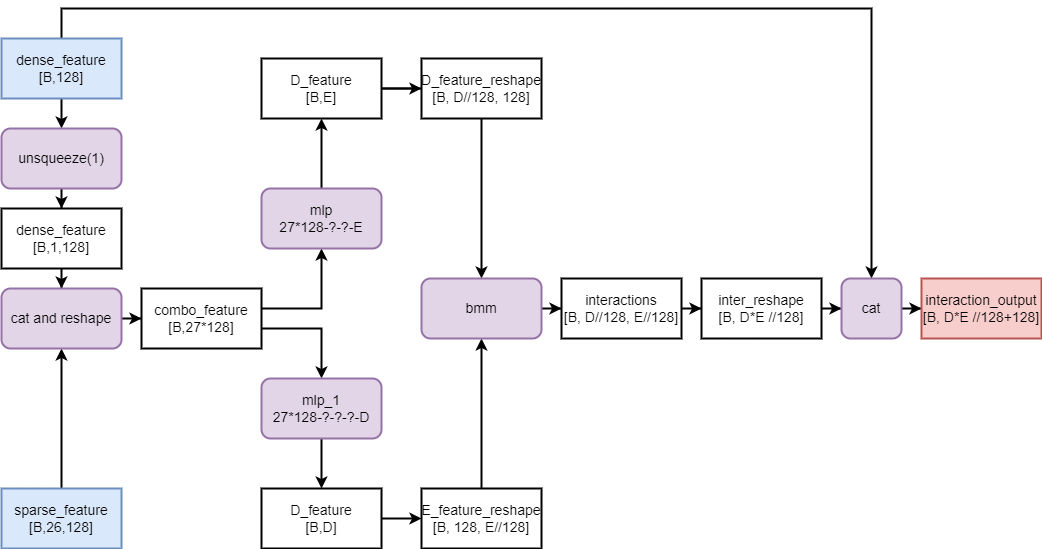
\includegraphics[scale=0.4]{dlrm2_projection.png}
    \caption{Projection Interaction}
\end{figure}

\end{document}


